\documentclass[tikz]{standalone}

\usetikzlibrary{positioning,shadows,arrows,trees}

\begin{document}
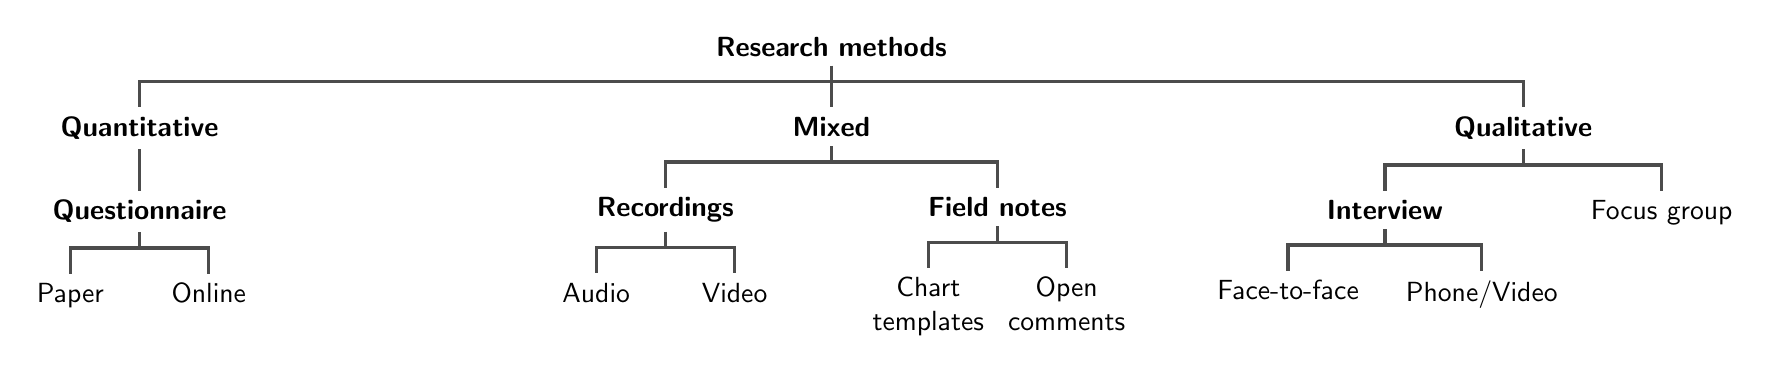
\begin{tikzpicture}[
	level distance=1.5em, 
  	edge from parent/.style={very thick,draw=black!70},
    edge from parent path={(\tikzparentnode.south) -- ++(0,-0.2cm) 
    	-|(\tikzchildnode.north)},
	growth parent anchor = south, 
	sibling distance = 25em]

\tikzstyle{branch} = [ 
    anchor = north, 
    align = center,
    font = \bfseries\sffamily
]
\tikzstyle{leaf} = [
    anchor=north, 
    align=center,
    font = \sffamily
]

\node [branch] {Research methods}
    child {[sibling distance = 0em] node [branch] {Quantitative}
		child {[sibling distance = 5em] node [branch] {Questionnaire}
			child { node [leaf] {Paper}}
			child { node [leaf] {Online}}
		}
	}			
	child {[sibling distance = 12em] node [branch] {Mixed}
		child {[sibling distance = 5em] node [branch] {Recordings}
			child { node [leaf] {Audio}}
			child { node [leaf] {Video}}
		}
		child {[sibling distance = 5em] node [branch] {Field notes}
			child { node [leaf] {Chart \\templates}}
			child { node [leaf] {Open\\ comments}}
		}			
	}
	child {[sibling distance = 10em] node [branch] {Qualitative}
		child {[sibling distance = 7em] node [branch] {Interview}
			child {node [leaf] {Face-to-face}}
			child {node [leaf] {Phone/Video}}
		} 
		child {node [leaf] {Focus group}}
	};
\end{tikzpicture}
\end{document}